\section{Dataset}

Per la valutazione dell'efficienza dell'algoritmo implementato è stato utilizzato una parte del dataset dell'\emph{ICPR HEp-2 Cell Classification Contest}.

Il dataset contiene al suo interno 149 immagini che rappresentano le scansioni di vetrini di laboratorio. All'interno di queste immagini è possibile distinguere 9 diversi pattern: \emph{punteggiato}, \emph{nucleolare}, \emph{citoplasmico}, \emph{omogeneo}, \emph{granulare}, \emph{negativo} e \emph{centromero}. Alcune immagini del dataset sono poi classificate come \emph{altro}, rendendo difficile una loro classificazione, questi elementi sono stati dunque non considerati. A causa del basso numero di elementi classificati con \emph{centromero} anche questi sono stati rimossi fino ad ottenere un totale di 137 immagini.

Le immagini sono state acquisite tramite un microscopio a fluorescenza (40 ingrandimenti) in combinazione con una lampada di mercurio vaporizzato a 50W e una fotocamera digitale SLIM con risoluzione 1920 x 1110.

\begin{figure}[H] 
  \centering
    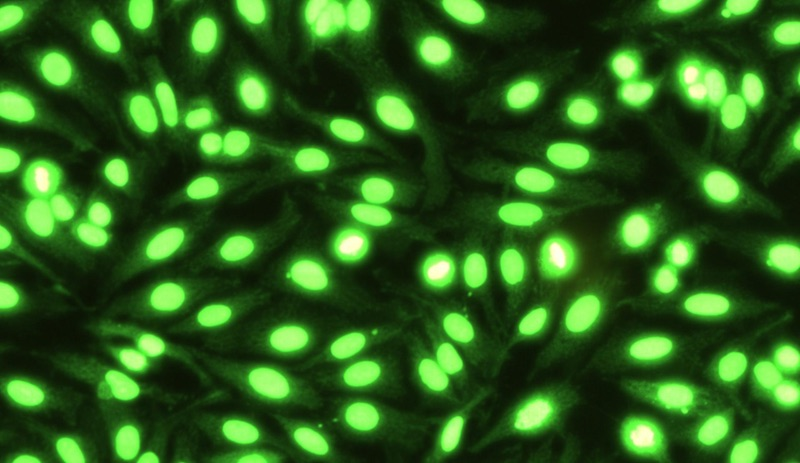
\includegraphics[width=0.9\textwidth]{images/example.jpg}
    \caption{{\small \textit{Esempio di immagine del dataset}}}
\end{figure}

Ciascuna immagine è stata poi annotata da un medico specialista ed associata ad una delle classi di pattern sopra esposte. Le annotazioni sono state inserite in una tabella così da poterne ricavare un \emph{training set}.

\begin{figure}[H]
\captionsetup[subfigure]{labelformat=empty}
\begin{subfigure}{.16\textwidth}
\centering
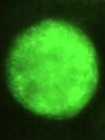
\includegraphics[height=1.6cm]{images/omogeneo.jpg}
\caption{Omogeneo}
\end{subfigure}%
\begin{subfigure}{.16\textwidth}
\centering
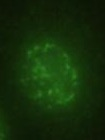
\includegraphics[height=1.8cm]{images/nucleolare.jpg}
\caption{Nucleolare}
\end{subfigure}%
\begin{subfigure}{.16\textwidth}
\centering
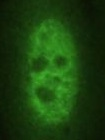
\includegraphics[height=1.8cm]{images/punteggiato.jpg}
\caption{Punteggiato}
\end{subfigure}%
\begin{subfigure}{.16\textwidth}
\centering
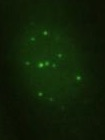
\includegraphics[height=1.8cm]{images/granulare.jpg}
\caption{Granulare}
\end{subfigure}%
\begin{subfigure}{.16\textwidth}
\centering
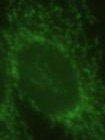
\includegraphics[height=1.8cm]{images/citoplasmico.jpg}
\caption{Citoplasmico}
\end{subfigure}%
\begin{subfigure}{.16\textwidth}
\centering

\includegraphics[height=1.8cm]{images/negativo.jpg}
\caption{Negativo}
\end{subfigure}%
\caption{Esempi di cellule classificate nel dataset}
\end{figure}
